\section{Auswertung}
\label{sec:Auswertung}
\subsection{Messdaten}
Die Daten wurden von der TU Dortmund bereitgestellt und aus dem Dokument \cite{DatenundHinweise} entnommen.
\begin{table}
  \centering
  \label{Aufgenommene Messdaten}
  \caption{Aufgenommene Messdaten}
  \begin{tabular}{S[table-format = 2.0] S[table-format = 2.1] S[table-format = 2.2] S[table-format = 2.1]
     S[table-format = 1.1] S[table-format = 3.0]}
     \toprule
     {$t \mathbin{/} \si{\second}$} & {$T_1 \mathbin{/} \si{\celsius}$} & {$p_1 \mathbin{/} \si{\bar}$} & {$T_2 \mathbin{/} \si{\celsius}$}
     & {$p_2 \mathbin{/} \si{\bar}$} & {$N \mathbin{/} \si{\watt}$} \\
     \midrule
     0	& 21.7 &	4.0    &	21.7 & 4.1 & 120 \\
     1  & 23.0 &	5.0    &	21.7 & 3.2 & 120 \\
     2 	& 24.3 &	5.5    &	21.6 & 3.4 & 120 \\
     3 	& 25.3 &	6.0    &	21.5 & 3.5 & 120 \\
     4 	& 26.4 &	6.0    &	20.8 & 3.5 & 120 \\
     5 	& 27.5 &	6.0    &	20.1 & 3.4 & 120 \\
     6 	& 28.8 &	6.5    &	19.2 & 3.3 & 120 \\
     7 	& 29.7 &	6.5    &	18.5 & 3.2 & 120 \\
     8 	& 30.9 &	7.0    &	17.7 & 3.2 & 120 \\
     9 	& 31.9 &	7.0    &	16.9 & 3.0 & 120 \\
    10	& 32.9 &	7.0    &	16.2 & 3.0 & 120 \\
    11	& 33.9 &	7.5    &	15.5 & 2.9 & 120 \\
    12	& 34.8 &	7.5    &	14.9 & 2.8 & 120 \\
    13	& 35.7 &	8.0    &	14.2 & 2.8 & 120 \\
    14	& 36.7 &	8.0    &	13.6 & 2.7 & 120 \\
    15	& 37.6 &	8.0    &	13.0 & 2.6 & 120 \\
    16	& 38.4 &	8.5    &	12.4 & 2.6 & 120 \\
    17	& 39.2 &	8.5    &	11.7 & 2.6 & 120 \\
    18	& 40.0 &	9.0    &	11.3 & 2.5 & 120 \\
    19	& 40.7 &	9.0    &	10.9 & 2.5 & 120 \\
    20	& 41.4 &	9.0    &	10.4 & 2.4 & 120 \\
    21	& 42.2 &	9.0    &	9.9	 & 2.4 & 120 \\
    22	& 42.9 &	9.5    &	9.5	 & 2.4 & 120 \\
    23	& 43.6 &	9.5    &	9.1	 & 2.4 & 120 \\
    24	& 44.3 &	10.0   &  8.7  & 2.4 & 120 \\
    25	& 44.9 &	10.0   &  8.3  & 2.4 & 120 \\
    26	& 45.5 &	10.0   &  8.0  & 2.3 & 120 \\
    27	& 46.1 &	10.0   &  7.7  & 2.2 & 122 \\
    28	& 46.7 &	10.5   &  7.4  & 2.2 & 122 \\
    29	& 47.3 &	10.5   &  7.1  & 2.2 & 122 \\
    30	& 47.8 &	10.75  &  6.8  & 2.2 & 122 \\
    31	& 48.4 &	11.0   &  5.6  & 2.2 & 122 \\
    32	& 48.9 &	11.0   &  4.3  & 2.2 & 122 \\
    33	& 49.4 &	11.0   &  3.4  & 2.2 & 122 \\
    34	& 49.9 &	11.0   &  3.0  & 2.2 & 122 \\
    35	& 50.3 &	11.0   &  2.9  & 2.2 & 122 \\
    \bottomrule 
  \end{tabular}
\end{table}
\newpage
\subsection{Temperaturverlauf mit Fit}
\begin{figure}
  \centering
  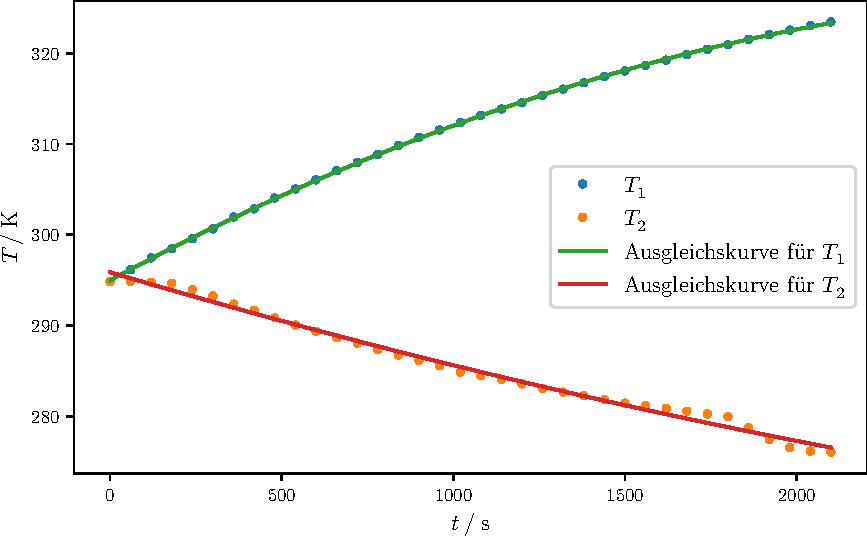
\includegraphics{temperatur.pdf}
  \caption{Temperaturverlauf beider Reservoirs.}
  \label{fig:temperatur}
\end{figure}
\subsection{Nicht-lineare Ausgleichsrechnung}
Der nicht-lineare Zusammenhang zwischen der Zeit und der Temperatur lässt sich mittels einer quadtratischen Ausgleichskurve, welche durch 
\begin{equation}
  T(t) = \symup{A}t^2 + \symup{B}t + \symup{C}
\end{equation}
beschrieben wird, approximieren. Mittels Rechnungen in numpy \cite{numpy} werden die Koeffizienten berechnet.
\begin{align}
  \intertext{Für T1 ergaben sich:}
  \symup{A}_1 &= \SI{-3.22(4)}{\micro\kelvin\per\second\tothe{2}} \\ 
  \symup{B}_1 &= \SI{20.28(9)}{\milli\kelvin\per\second} \\
  \symup{C}_1 &= \SI{294.97(4)}{\kelvin}  \\
  \intertext{für T2:}
  \symup{A}_2 &= \SI{0.95(7)}{\micro\kelvin\per\second\tothe{2}}\\
  \symup{B}_2 &= \SI{-11.21(10)}{\milli\kelvin\per\second}\\
  \symup{C}_2 &= \SI{295.87(26)}{\kelvin}
\end{align}
\subsection{Differentialquotient}
Der Differentialquotient der approximierenden Funktion ist durch
\begin{equation}
  \frac{\symup{d} T(t)}{\symup{d}t} = 2\symup{A}t + \symup{B}  
\end{equation}
gegeben. Die in die Differentialquotienten eingesetzen Zeitpunkte $t = 600s$, $t = 900$, $t = 1200$ und $t = 2100$ ergeben folgende Tabelle:
\begin{table}
  \centering
  \caption{Ergebnisse der Differentialquotienten}
  \label{tab:Differentialquotient}
  \sisetup{table-format = 1.4}
  \begin{tabular}{S[table-format = 4.0] S[table-format = 2.2] @{${}\pm{}$} S[table-format = 0.2] S[table-format= 3.2] @{${}\pm{}$} S[table-format = 0.2]}
    \toprule
    {$t \mathbin{/} \si{\second}$} & \multicolumn{2}{c}{$\frac{\symup{d} T_1}{\symup{d}t} \mathbin{/} \si{\milli\kelvin\second\tothe{-1}}$}
    & \multicolumn{2}{c}{$\frac{\symup{d} T_2}{\symup{d}t} \mathbin{/} \si{\milli\kelvin\second\tothe{-1}}$} \\
    \cmidrule(lr){2-3} \cmidrule(lr){4-5}
    \midrule
    600  & 16.42 & 0.10 & -10.07 & 0.13\\
    900  & 14.48 & 0.12 & -9.50  & 0.16\\
    1200 & 12.55 & 0.13 & -8.93  & 0.20\\
    2100 & 67.56 & 0.19 & -7.22  & 0.31\\
    \bottomrule
  \end{tabular}
\end{table}
\subsection{Güteziffer}
Um die reale Güteziffer zu bestimmen dient die Gleichung \eqref{eqn:Güteziffer}.
Für die Wärmekapazität des Wassers (Masse: $m_\text{w} = \SI{4}{\kilo\gram}$ \cite{DatenundHinweise}, 
Spezifische Wärmekapazität: $c_\text{w} = \SI{4.186}{\kilo\joule\per\kilo\gram\per\kelvin}$ \cite{spezWärmeKap})
gilt $m_1 c_\text{w} = \SI{16744}{\joule\per\kelvin}$,
für die der Kupferschlangen $m_\text{k}c_\text{k} = \SI{750} {\joule\per\kelvin}$ \cite{DatenundHinweise}. Für die Berechnung der idealen Güterziffer $\nu_\text{id}$ ist die Beziehung \eqref{eqn:Id} von Nutzen.
Mittels Rechnungen ergaben sich die Werte der Güterziffern zu:
\begin{table}
  \centering
  \caption{Vergleich $\nu_\text{re}$ zu $\nu_\text{id}$}
  \label{tab:Gueterziffer}
  \sisetup{table-format = 2.4}
  \begin{tabular}{S[table-format = 4.0] S[table-format = 1.2] @{${}\pm{}$} S[table-format = 0.2] S[table-format = 2.2] @{${}\pm{}$} S[table-format = 0.2] 
    S[table-format = 2.2] @{${}\pm{}$} S[table-format = 0.2]}
    \toprule
    {$t \mathbin{/} \si{\second}$} & \multicolumn{2}{c}{$\nu_\text{re}$} & \multicolumn{2}{c}{$\nu_\text{id}$}  
    & \multicolumn{2}{c}{$\frac{\nu_\text{re}} {\nu_\text{id}} \si{\percent}$} \\
    \cmidrule(lr){2-3} \cmidrule(lr){4-5} \cmidrule(lr){6-7}
    \midrule
     600  & 2.39 & 0.01 & 18.32 & 0.30 & 13.04 & 0.22\\
     900  & 2.11 & 0.02 & 12.63 & 0.14 & 16.69 & 0.23\\    
    1200  & 1.83 & 0.02 & 10.15 & 0.09 & 18.00 & 0.25\\  
    2100  & 0.97 & 0.03 &  6.82 & 0.04 & 14.17 & 0.41\\    
    \bottomrule                                       
  \end{tabular}                                     
\end{table}
\subsection{Massendurchsatz}
Der Massendurchsatz lässt sich mittels Gleichung \eqref{eqn:Massendurchsatz} ermitteln, jedoch fehlt zunächst der Wert der Verdampfungswärme L, welche 
mit Hilfe einer Dampfdruck-Kurve gewonnen werden kann. Diese Kurve wird durch 
\begin{equation}
  \ln (p) = -\frac{L}{\symup{R}T} + \symup{const} \label{eqn:Verdampfungswaerme}
\end{equation}
beschrieben, wobei R die allgemeine Gaskonstante ist. Zwecks der Definition $a \coloneq -\frac{L}{\symup{R}}$ erhält man die Vereinfachung
\begin{equation}
  \ln (p) = \frac{a}{T} + \symup{const}
\end{equation}
\begin{figure}
  \centering
  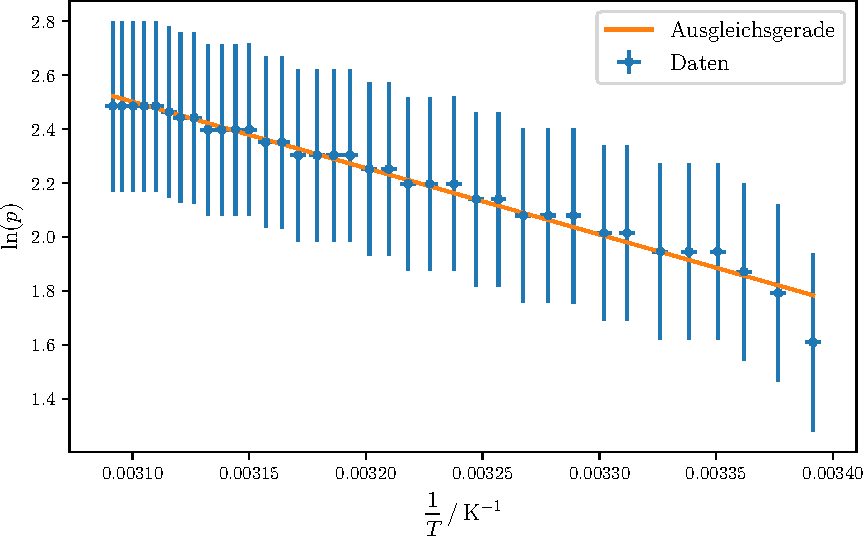
\includegraphics{Verdampfungswaerme.pdf}
  \caption{Dampfdruck-Kurve}
  \label{fig:Dampfdruck}
\end{figure}
Hierbei ist zu beachten, dass das Argument des natürlichen Logarithmus nicht einheitslos ist (was normalerweise
der Fall sein müsste), da die Gleichung \eqref{eqn:Verdampfungswaerme} durch Vereinfachungen angenähert wurde.
Nach der Durchführung der linearen Regression, erhält man, dass $a = \SI{-2462.4863(705436)}{\kelvin}$ gilt und der Wert der Konstante zu $\num{10.1354(2268)}$ ist.
Rücksubstituieren von $a = -\frac{L}{\symup{R}}$ und umstellen nach $L$ führt zu $ L = - \symup{R}a$. Einsetzen von $a$ und der allgemeinen Gaskonstante 
$\symup{R} = \SI{8.314462}{\joule\per\mole\per\kelvin}$ \cite{allgGaskonstante} liefert
\begin{equation}
  L = \SI{20500(600)}{\joule\per\mol}\, .
\end{equation}
Um die Einheit von $\si{\joule\per\mole}$ auf Energie pro Masse, also $\si{\joule\per\gram}$ umzurechnen, dividiert man durch die Molare
Masse von Dichlordifluormethan ($M = \SI{120.91}{\gram\per\mole}$), sodass man letzendlich
\begin{equation}
  L = \SI{169(5)}{\joule\per\gram}
\end{equation}
erhält.
Nach der Bestimmung der Verdampfungswärme kennt man alle Größen, so dass die Berechnung des Massendurchsatzes folgt.
\begin{table}
  \centering
  \caption{Ergebnisse des Massendurchsatzes}
  \label{tab:Massendurchsatz}
  \begin{tabular}{S[table-format = 4.0] S[table-format = 3.2] @{${}\pm{}$} S[table-format = 0.2] S[table-format= 2.2] @{${}\pm{}$} S[table-format = 0.2]}
    \toprule
    {$t \mathbin{/} \si{\second}$} & \multicolumn{2}{c}{$\frac{\symup{d} T_2}{\symup{d}t} \mathbin{/} \si{\milli\kelvin\second\tothe{-1}}$}
    & \multicolumn{2}{c} {$\frac{\symup{d} m_2}{\symup{d}t} \mathbin{/} \si{\gram\second\tothe{-1}}$} \\
    \cmidrule(lr){2-3} \cmidrule(lr){4-5}
    \midrule
    600  & -10.07 & 0.13 & -1.04 & 0.03\\
    900  & -9.50  & 0.16 & -0.98 & 0.03\\
    1200 & -8.93  & 0.20 & -0.92 & 0.03\\
    2100 & -7.22  & 0.31 & -0.75 & 0.04\\
    \bottomrule
  \end{tabular}
\end{table}
\subsection{Mechanische Kompressorleistung}
Um die mechanische Kompressorleistung zu bestimmen, wird die Gleichung \eqref{eqn:Kompressor} benötigt. Bevor man aber mit der Berechnung fortfahren kann, benötigt
man noch die Dichte des Transportmediums $\rho$. Diese lässt sich mittels der idealen Gasgleichung \eqref{eqn:gasgleichung} errechnen. Für die gemessenen Werte 
$p_1$, $p_2$ und $T_2$, die gegebenen Werte $\rho_0 = \SI{5.51}{\gram\per\liter}$, $p_0 = \SI{1}{\bar}$ und $T_0 = \SI{273.15}{\kelvin}$ \cite{DatenundHinweise}
ergaben sich für Dichte des Mediums, die in der Tabelle 
\eqref{tab:Mechanische Kompressorleistung} stehenden, Werte.
Anschließend erhält man die mechanische Kompressorleistung als:
\begin{table}
  \centering
  \caption{Errechnete mechanische Kompressorleistung}
  \label{tab:Mechanische Kompressorleistung}
  \begin{tabular}{S[table-format = 4.0] S[table-format = 2.1] S[table-format = 1.1] S[table-format= 2.2] @{${}\pm{}$} S[table-format = 0.2] S[table-format = 2.2]
    @{${}\pm{}$} S[table-format = 0.2]}
    \toprule
    {$t \mathbin{/} \si{\second}$} & {$p_ 1 \mathbin{/} \si{bar}$} & {$p_ 2 \mathbin{/} \si{bar}$} & \multicolumn{2}{c}{$\rho \mathbin{/} \si{\gram\liter\tothe{-1}}$} 
    & \multicolumn{2}{c}{$N_\text{mech} \mathbin{/} \si{\watt}$}\\
    \cmidrule(lr){4-5} \cmidrule(lr){6-7}
    \midrule
     600 &  8.0 & 4.0 & 20.81 & 0.01 & 12.70 & 0.41\\
     900 &  9.0 & 3.6 & 18.93 & 0.01 & 15.88 & 0.54\\    
    1200 & 10.0 & 3.4 & 18.05 & 0.01 & 17.59 & 0.65\\  
    2100 & 12.0 & 3.2 & 17.45 & 0.01 & 17.22 & 0.90\\    
    \bottomrule                                       
  \end{tabular}                                     
\end{table}
\subsection{Fehlerrechnung}
Jegliche Fehlerrechnung wurde mit Hilfe der Python-Bibliothek Uncertainties \cite{uncertainties} automatisiert und effizient absolviert.